\let\lesson\undefined
\newcommand{\lesson}{\phantomlesson{Bài 23: Biến dạng của vật rắn. Đặc tính của lò xo. Định luật Hooke}}
\chapter[Biến dạng của vật rắn. Đặc tính của lò xo\\ Định luật Hooke]{Biến dạng của vật rắn. Đặc tính của lò xo\\ Định luật Hooke}
\setcounter{section}{0}
\section{Lý thuyết}
\subsection{Biến dạng kéo và biến dạng nén}
Khi không có ngoại lực tác dụng, vật rắn có kích thước và hình dạng xác định. Khi có ngoại lực tác dụng, vật rắn thay đổi hình dạng và kích thước, ta nói vật rắn bị biến dạng.

\begin{minipage}{0.6\textwidth}
	\subsubsection{Biến dạng kéo}
	Dấu hiệu: Kích thước của vật theo phương tác dụng của lực tăng lên so với kích thước tự nhiên của nó.
	\subsubsection{Biến dạng nén}
	Dấu hiệu: Kích thước của vật theo phương tác dụng của lực giảm xuống so với kích thước tự nhiên của nó.
\end{minipage}
\begin{minipage}{0.4\textwidth}
	\begin{center}
		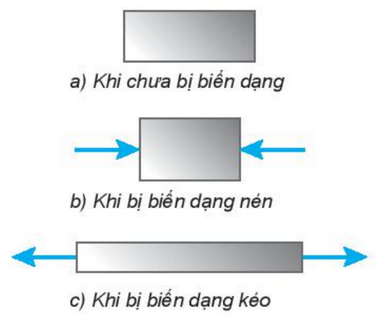
\includegraphics[scale=0.6]{../figs/G10-028-1}
	\end{center}
\end{minipage}
\subsection{Biến dạng đàn hồi}
Khi không còn tác dụng của ngoại lực, nếu vật rắn lấy lại được kích thước và hình dạng ban đầu thì biến dạng của vật là biến dạng đàn hồi.

Giới hạn mà trong đó vật rắn còn giữ được tính đàn hồi được gọi là giới hạn đàn hồi của vật rắn.
\begin{center}
	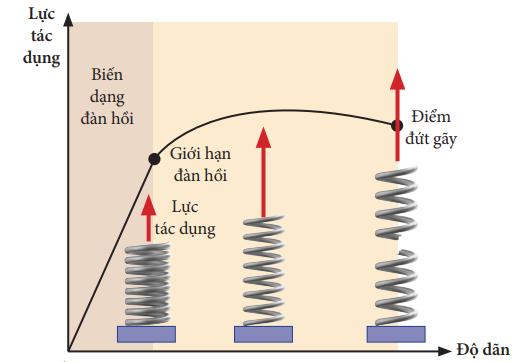
\includegraphics[width=0.45\linewidth]{../figs/VN10-2023-PH-TP033-1}
	\captionof{figure}{Đồ thị biểu diễn mối liên hệ giữa độ dãn lò xo và lực tác dụng.}
\end{center}

\subsection{Đặc tính của lò xo}
Các loại lò xo đều có tính đàn hồi. Lò xo bị biến dạng kéo hoặc biến dạng nén tùy thuộc vào chiều của lực đặt vào hai đầu lò xo.

\begin{minipage}{0.6\textwidth}
	Độ biến dạng của lò xo (kí hiệu: $\Delta \ell$) là hiệu số giữa chiều dài khi bị biến dạng và chiều dài tự nhiên của lò xo:
	$$\Delta \ell=\ell-\ell_0$$
	\begin{itemize}
		\item Khi lò xo biến dạng nén: độ biến dạng của lò xo âm, độ lớn của độ biến dạng được gọi là độ nén.
		\item Khi lò xo biến dạng kéo: độ biến dạng của lò xo dương và được gọi là độ dãn.
	\end{itemize}
	
	
	Khi hai lò xo chịu tác dụng bởi hai lực kéo/nén có độ lớn bằng nhau và đang bị biến dạng đàn hồi, lò xo có độ cứng lớn hơn sẽ bị biến dạng ít hơn.
\end{minipage}
\begin{minipage}{0.4\textwidth}
	\begin{center}
		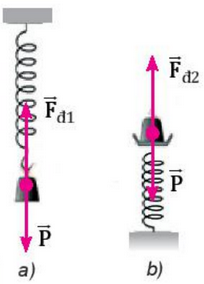
\includegraphics[scale=0.8]{../figs/G10-028-2}
	\end{center}
\end{minipage}

\subsection{Định luật Hooke}
\begin{minipage}{0.6\textwidth}
	
	Khi lò xo bị biến dạng, trong lò xo xuất hiện lực đàn hồi có xu hướng chống lại sự biến dạng. 			
	
	Trong giới hạn đàn hồi, độ lớn của lực đàn hồi của lò xo tỉ lệ thuận với độ biến dạng của lò xo.
	\begin{equation*}
		F= k \cdot |\Delta \ell|.
	\end{equation*}
	
	Trong đó:
	\begin{itemize}
		\item $k$ là độ cứng của lò xo (N/m). Hệ số $k$ càng lớn thì lò xo càng ít bị biến dạng. Độ cứng của lò xo phụ thuộc vào chất thép dùng làm lò xo, đường kính của vòng xoắn và tiết diện
		dây.
		\item $|\Delta \ell|=|\ell-\ell_0|$ là độ biến dạng của lò xo (m).
		\item $F$ là lực đàn hồi của lò xo (N).
	\end{itemize}
\end{minipage}
\begin{minipage}{0.4\textwidth}
	\begin{center}
		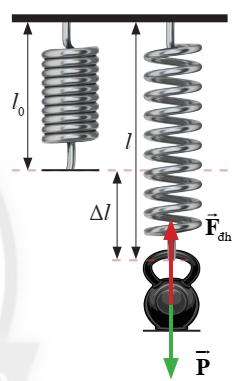
\includegraphics[scale=0.65]{../figs/G10-028-5}
	\end{center}
	
\end{minipage}
\subsection{Ứng dụng định luật Hooke}
\begin{minipage}{0.6\textwidth}
	Cân đồng hồ (hay còn gọi là cân đồng hồ lò xo) là loại cân được sử dụng nhiều trong đời sống. Cân đồng hồ lò xo bao gồm loại để bàn và loại có móc treo.
	
	Cân hoạt động dựa trên sự biến dạng của lò xo, tạo trạng thái cân bằng khi lò xo chịu tác dụng nén (cân đĩa) hoặc kéo (cân móc treo). Trên cân có bộ phận chuyển đổi chuyển động thẳng (do kéo  hoặc nén) của lò xo sang chuyển động xoay tròn của kim chỉ thị và hiển thị kết quả đo trên mặt số của đồng hồ.
\end{minipage}
\begin{minipage}{0.4\textwidth}
	\begin{center}
		
\includegraphics[scale=0.5]{../figs/G10-028-3}
	\end{center}
\end{minipage}

\section{Mục tiêu bài học - Ví dụ minh họa}
\begin{dang}{Nêu khái niệm biến dạng đàn hồi, biến dạng kéo và biến dạng nén}
	\viduii{1}{Kích thước và hình dạng của vật khi biến dạng kéo và biến dạng nén khác nhau như thế nào?
	}
	{	\begin{center}
			\textbf{Hướng dẫn giải}
		\end{center}
		
		\begin{itemize}
			\item Biến dạng kéo: Kích thước của vật theo phương tác dụng của lực tăng lên so với kích thước tự nhiên của nó.
			
			\item Biến dạng nén: Kích thước của vật theo phương tác dụng của lực giảm xuống so với kích thước tự nhiên của nó.
		\end{itemize}
	}
	\viduii{1}{Trong thí nghiệm với lò xo và vòng dây cao su, nếu lực kéo quá lớn thì khi thôi tác dụng lực, chúng có trở về hình dạng, kích thước ban đầu được không?
	}
	{	\begin{center}
			\textbf{Hướng dẫn giải}
		\end{center}
		
		Khi tăng cường độ lực tác dụng, độ giãn của lò xo và vòng dây cao su tăng. Tuy nhiên, khi tăng giá trị lực vượt quá một giới hạn nào đó thì khi dừng tác dụng lực, lò xo sẽ không thể chiều dài ban đầu nữa, hoặc vòng dây cao su sẽ bị đứt. Giá trị giới hạn này được gọi là giới hạn đàn hồi.
	}
	\viduii{2}{Tìm hiểu và giải thích tại sao ở Nhật Bản, nhiều tòa nhà cao tầng được xây dựng với các lò xo ở dưới móng cọc.
	}
	{	\begin{center}
			\textbf{Hướng dẫn giải}
		\end{center}
		
		Ở Nhật Bản, các tòa nhà khi được xây dựng đều phải tuân theo những tiêu chuẩn chống động đất rất khắt khe. Một trong số đó là việc có các lò xo ở dưới móng cọc. Mục đích của việc này là để lò xo hấp thụ xung lực từ các chấn động và giảm xóc cho tòa nhà.
	}
\end{dang}
\begin{dang}{Nhận biết đặc điểm của lực đàn hồi của lò xo. Ghi nhớ định luật Hooke}
	\viduii{1}{Lực đàn hồi xuất hiện tỉ lệ với độ biến dạng khi 
		\begin{mcq}
			\item một vật bị biến dạng dẻo.
			\item một vật biến dạng đàn hồi.
			\item một vật bị biến dạng.	
			\item ta ấn ngón tay vào một viên đất nặn.
		\end{mcq}
	}
	{	\begin{center}
			\textbf{Hướng dẫn giải}
		\end{center}
		
		Lực đàn hồi xuất hiện tỉ lệ với độ biến dạng khi một vật biến dạng đàn hồi.
		
		\textbf{Đáp án: B}.
	}
	\viduii{1}{Điều nào sau đây là \textbf{sai}?
		\begin{mcq}
			\item Độ cứng của lò xo cũng được gọi là hệ số đàn hồi của lò xo.
			\item Lò xo có độ cứng càng nhỏ càng khó biến dạng.
			\item Độ cứng cho biết sự phụ thuộc tỉ lệ của độ biến dạng của lò xo vào lực gây ra sự biến dạng đó.
			\item Độ cứng phụ thuộc hình dạng, kích thước lò xo và chất liệu làm lò xo.
		\end{mcq}
	}
	{	\begin{center}
			\textbf{Hướng dẫn giải}
		\end{center}
		
		Lò xo có độ cứng càng lớn càng khó biến dạng.
		
		\textbf{Đáp án: B}.
	}
\end{dang}
\begin{dang}{Tính độ biến dạng của lò xo và các đại lượng trong định luật Hooke}
	\viduii{2}{Một quả cân có khối lượng $m = \SI{100}{g}$ treo vào đầu dưới của một lò xo nhẹ, đầu kia của lò xo gắn trên giá treo. Cho $g= \SI{10}{m/s^2}$. Khi vật cân bằng thì lực của lò xo tác dụng lên vật là bao nhiêu?
	}
	{	\begin{center}
			\textbf{Hướng dẫn giải}
		\end{center}
		
		\begin{itemize}
			\item Vật chịu tác dụng của trọng lực $\vec{P}$ và lực đàn hồi $\vec{F}_{\text{đh}}$.
			\item Khi vật nằm cân bằng
			\begin{equation*}
				F_{\text{đh}} = P = mg =\SI{1}{N}.
			\end{equation*}
		\end{itemize}
	}
	
	\viduii{3}{Một lò xo có chiều dài tự nhiên là $\SI{30}{cm}$, khi bị nén dọc theo trục lò xo với lực có độ lớn $\SI{5}{\newton}$ thì lò xo có chiều dài $\SI{24}{\centi\meter}$. Hỏi khi lò xo bị nén bằng lực  $\SI{10}{N}$ thì chiều dài của nó bằng bao nhiêu?
	}
	{	\begin{center}
			\textbf{Hướng dẫn giải}
		\end{center}
		Độ cứng của lò xo
		\begin{equation*}
			k = \dfrac{F}{\left|\Delta\ell\right|} =\dfrac{\SI{5}{\newton}}{\SI{6E-2}{\meter}}=\xsi{\dfrac{250}{3}}{\newton/\meter}
		\end{equation*}
		Độ biến dạng của lò xo khi bị nén với lực $\SI{10}{\newton}$
		\begin{equation*}
			\left|\Delta \ell'\right| =\dfrac{F'}{k} =\dfrac{\SI{10}{\newton}}{\xsi{\dfrac{250}{3}}{\newton/\meter}}= \SI{0,12}{\meter}=\SI{12}{\centi\meter}.
		\end{equation*}
		Chiều dài của lò xo lúc này
		\begin{equation*}
			\ell'=\ell_0 -\left|\Delta \ell\right| = \SI{18}{cm}.
		\end{equation*} 
		
	}
	
	
	\viduii{3}{Một lò xo có chiều dài tự nhiên bằng $\SI{20}{cm}$ được treo thẳng đứng vào một điểm cố định. Khi treo vào đầu còn lại một vật có khối lượng $\SI{500}{g}$, lò xo có chiều dài $\SI{22}{cm}$ khi vật ở vị trí cân bằng. Lấy $g=\SI{9.8}{m/s^2}$.
		\begin{enumerate}[label=\alph*)]
			\item Tính độ cứng của lò xo.
			\item Để giữ vật nặng cố định tại vị trí lò xo có chiều dài bằng $\SI{19}{cm}$, cần tác dụng một lực nâng vào vật theo phương thẳng đứng có độ lớn bằng bao nhiêu?
		\end{enumerate}
	}
	{	\begin{center}
			\textbf{Hướng dẫn giải}
		\end{center}
		
		\begin{enumerate}[label=\alph*)]
			\item Tính độ cứng của lò xo.
			\begin{center}
				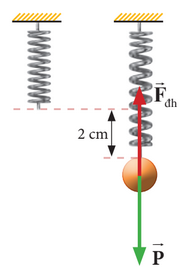
\includegraphics[scale=0.6]{../figs/G10-028-4}
			\end{center}
			
			Độ dãn của lò xo khi vật ở vị trí cân bằng:
			$$\Delta \ell = \ell - \ell_0 = \SI{22}{\centi\meter} - \SI{20}{\centi\meter} = \SI{2}{\centi\meter}=\SI{0.02}{\meter}.$$
			Khi này, lực đàn hồi của lò xo cân bằng với trọng lực của vật như phân tích lực trong hình bên:
			$$F_\text{đh} = m g = \SI{0.5}{\kilogram} \cdot \SI{9.8}{\meter/\second^2} = \SI{4.9}{N}$$
			Vậy độ cứng của lò xo:
			$$k=\dfrac{F}{\Delta \ell} = \dfrac{\SI{4.9}{\newton}}{\SI{0.02}{\meter}} = \SI{245}{N/m}$$
			
			\item Tại vị trí lò xo có chiều dài bằng $\SI{19}{cm}$, có ba lực tác dụng vào vật theo phương thẳng đứng: trọng lực có chiều hướng xuống; lực đàn hồi của lò xo lúc này có chiều hướng xuống vì lò xo bị nén so với chiều dài tự nhiên và lực nâng hướng lên.
			
			Khi này, lực đàn hồi có độ lớn:
			$$F_\text{đh} = k |\Delta \ell| = \SI{245}{\newton/\meter} \cdot |\SI{0.19}{\meter} - \SI{0.2}{\meter}| = \SI{2.45}{\newton}$$
			
			Do vật đứng yên nên lực tổng hợp tác dụng vào vật triệt tiêu, suy ra lực nâng của tay có độ lớn:
			$$F=m  g + F_\text{đh} =\SI{0.5}{\kilogram}\cdot\SI{9.8}{\meter/\second^2} + \SI{2.45}{\newton} = \SI{7.35}{\newton}$$
		\end{enumerate}
		
		\begin{center}
			\textbf{Câu hỏi tương tự}
		\end{center}
		
		Một lò xo bố trí theo phương thẳng đứng và có gắn vật nặng khối lượng $\SI{200}{g}$. Khi vật treo ở dưới thì lò xo dài $\SI{17}{cm}$, khi vật đặt ở trên thì lò xo dài $\SI{13}{cm}$. Lấy $g=\SI{10}{m/s^2}$ và bỏ qua trọng lượng của móc treo, giá đỡ vật nặng. Tính độ cứng của lò xo.
		
		\textbf{Đáp án:} $k=\SI{100}{N/m}$.
	}
\end{dang}